\subsubsection{rendering.tick.dynamics}
    Enthält Klassen um \textit{DynamicGameObject}s auf Nodes im Scenegraph der JMonkeyEngine anzuwenden.\par

    \begin{figure}[htbp]
        \centering
        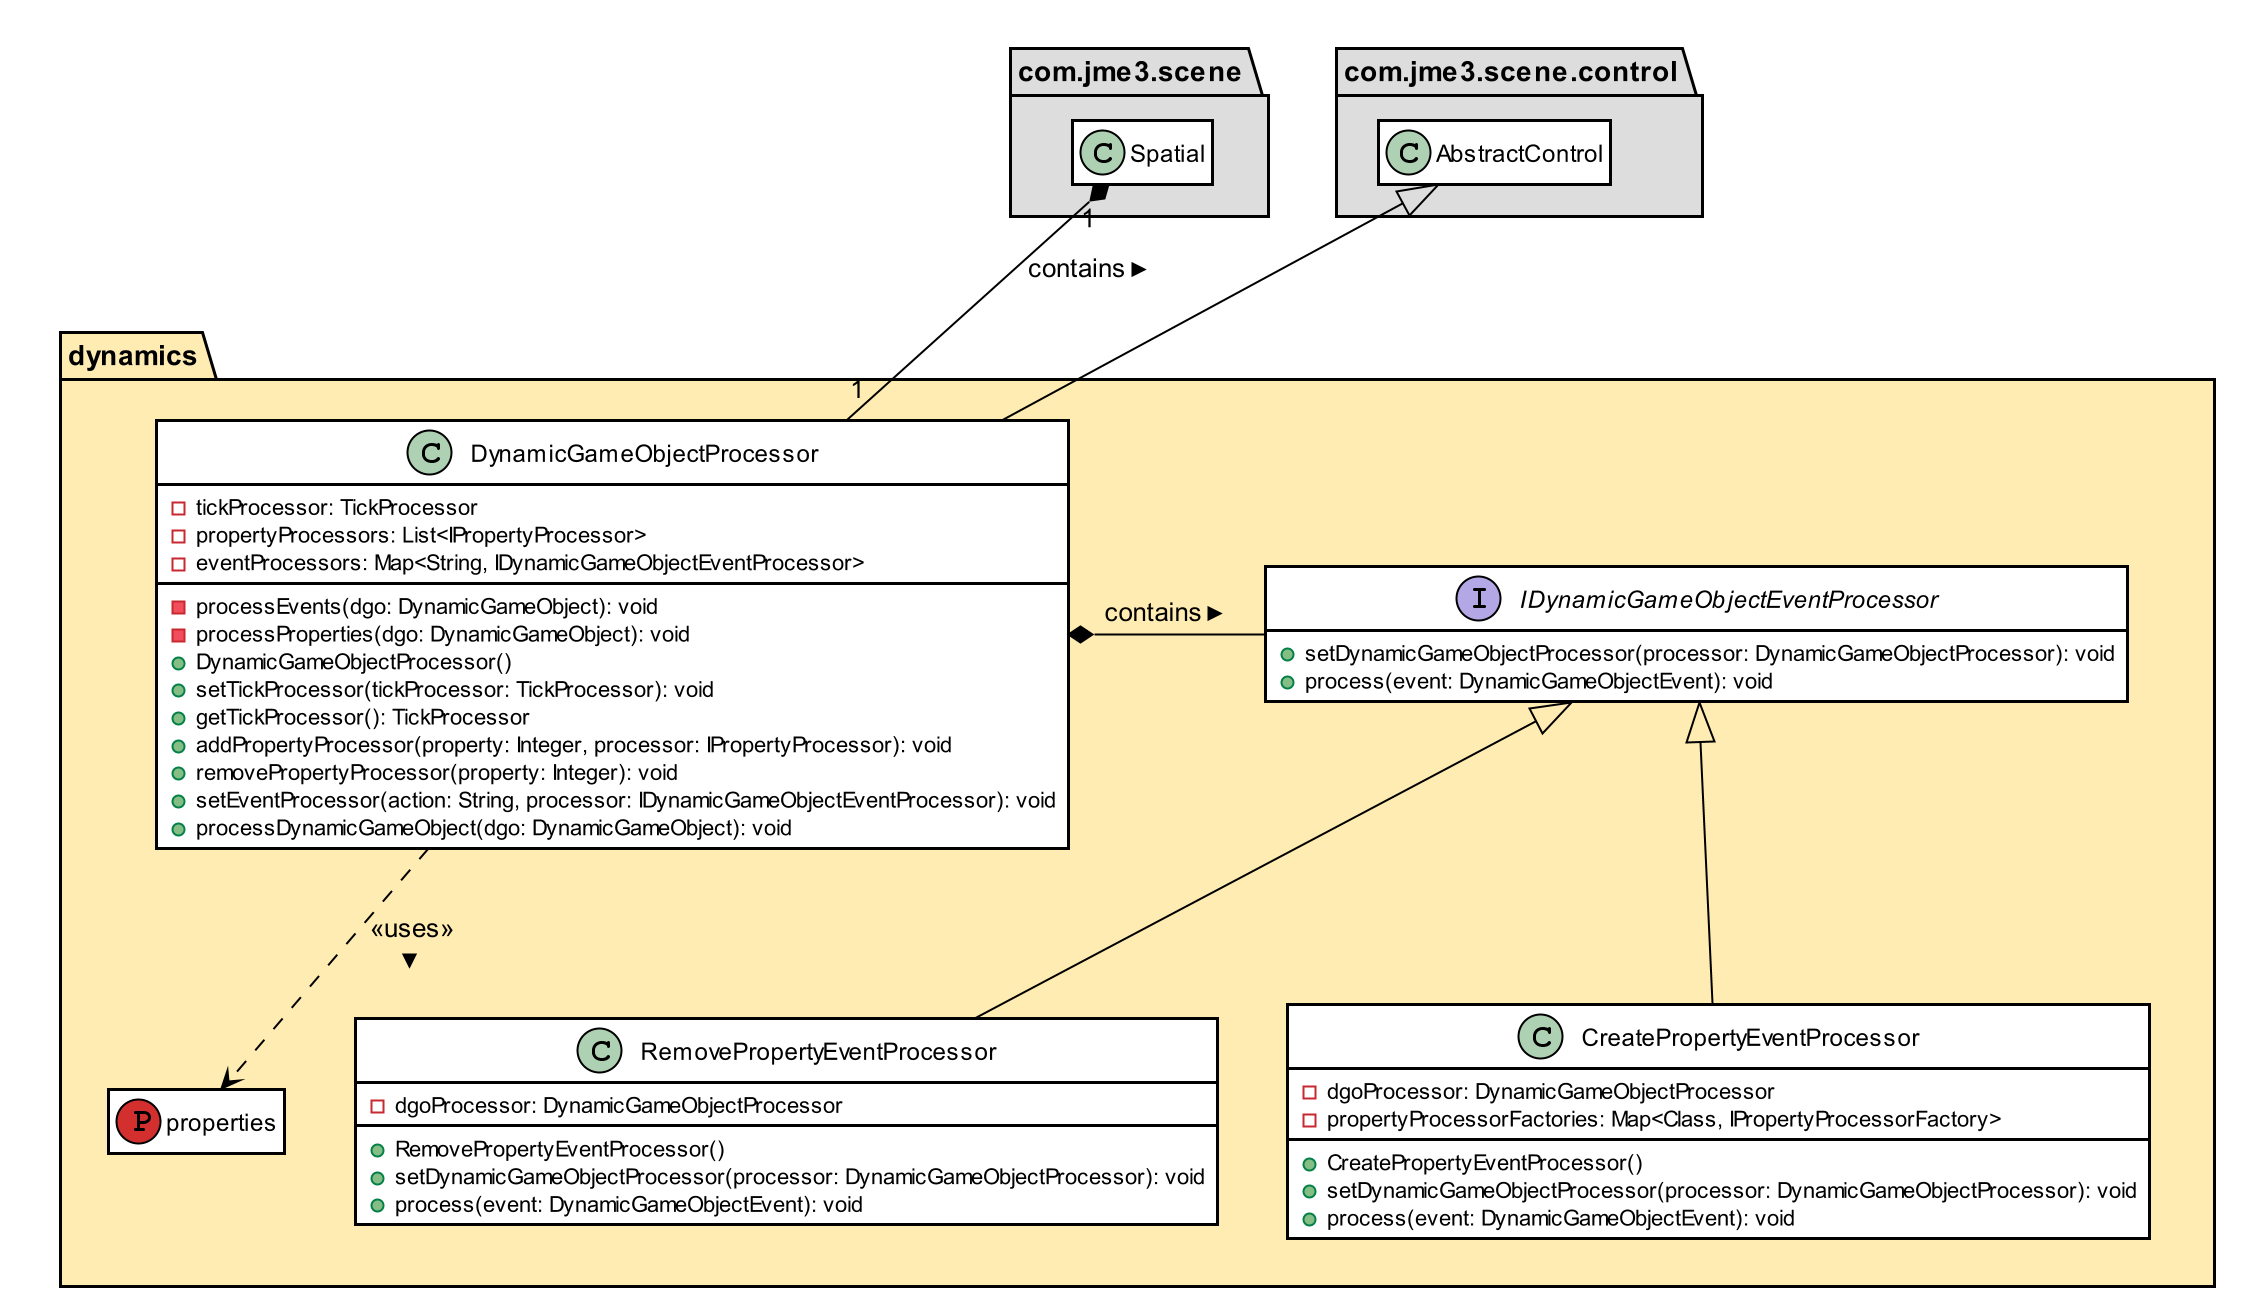
\includegraphics[width=\linewidth]{Interface/render-tick-dynamics.png}
        \caption{rendering.tick.dynamics Klassen-Diagram}
    \end{figure}

        \paragraph{\underline{DynamicGameObjectProcessor}} \mbox{}\\
        \\
            Verarbeitet \textit{DynamicGameObject}s indem er die in diesem enthaltenen \textit{IProperty}s an
            \textit{IPropertyProcessor}s weiterleitet und \textit{DynamicGameObjectEvent}s mit den zugehörigen \textit{IDynamicGameObjectEventProcessor}s bearbeitet.\par
                    
            \textbf{Attribute}
            \begin{itemize}
                \item  \textit{- TickProcessor tickProcessor}
                    \begin{leftbar}[0.9\linewidth]
                        Der \textit{TickProcessor}, welcher diesen \textit{DynamicGameObjectProcessor} verwendet.
                    \end{leftbar}
                \item \textit{- List<IPropertyProcessor> propertyProcessors}
                    \begin{leftbar}[0.9\linewidth]
                        Enthält alle momentan bekannten \textit{IPropertyProcessor}s.
                    \end{leftbar}
                \item \textit{- Map<String, IDynamicGameObjectEventProcessor> eventProcessors}
                    \begin{leftbar}[0.9\linewidth]
                        Enthält für jede benötigte Aktion eines \textit{DynamicGameObjectEvent}s einen \textit{IDynamicGameObjectEventProcessor}.
                    \end{leftbar}
            \end{itemize}

            \pagebreak
            \textbf{Methoden}
            \begin{itemize}
                \item \textit{+ DynamicGameObjectProcessor()}
                    \begin{leftbar}[0.9\linewidth]
                        Erstellt einen neuem \textit{DynamicGameObjectProcessor} und initialisiert propertyProcessors als leere List
                        und eventProcessors als leere Map.
                    \end{leftbar}
                \item \textit{+ setTickProcessor(TickProcessor tickProcessor): void}
                    \begin{leftbar}[0.9\linewidth]
                        Setzt den \textit{TickProcessor}, welcher diesen \textit{DynamicGameObjectProcessor} aufruft.\\
                        \textbf{@param tickProcessor} der \textit{TickProcessor}, welcher diesen \textit{DynamicGameObjectProcessor} aufruft.
                    \end{leftbar}
                \item \textit{+ getTickProcessor(): TickProcessor}
                    \begin{leftbar}[0.9\linewidth]
                        \textbf{@return} den \textit{TickProcessor}, welcher diesen \textit{DynamicGameObjectProcessor} aufruft.
                    \end{leftbar}
                \item \textit{+ addPropertyProcessor(int property, IPropertyProcessor processor): void}
                    \begin{leftbar}[0.9\linewidth]
                        Fügt einen \textit{IPropertyProcessor} für die \textit{IProperty} mit dem gegebenen index hinzu.\\
                        \textbf{@param property} der index der \textit{IProperty}.\\
                        \textbf{@param processor} der \textit{IPropertyProcessor}, wecher hinzugefügt werden soll.
                    \end{leftbar}
                \item \textit{+ removePropertyProcessor(int property): void}
                    \begin{leftbar}[0.9\linewidth]
                        Entfernt \textit{IPropertyProcessor} für die \textit{IProperty} mit dem gegebenen index.\\
                        \textbf{@param property} der index der \textit{IProperty}.
                    \end{leftbar}
                \item \textit{+ setEventProcessor(String action, IDynamicGameObjectEventProcessor processor): void}
                    \begin{leftbar}[0.9\linewidth]
                        Setzt den \textit{IDynamicGameObjectEvenProcessor} für \textit{DynamicGameObjectEvent}s mit der gegebenen Aktion.\\
                        \textbf{@param action} die Aktion für die der \textit{IDynamicGameObjectEvenProcessor} gesetzt werden soll.
                        \textbf{@param processor} der \textit{IDynamicGameObjectEvenProcessor}
                    \end{leftbar}
                \item \textit{+ processBundle(DynamicGameObject dgo): void}
                    \begin{leftbar}[0.9\linewidth]
                        Verarbeitet das gegebene \textit{DynamicGameObject}.\\
                        \textbf{@param dgo} das \textit{DynamicGameObject}, das verarbeitet werden soll.
                    \end{leftbar}
            \end{itemize}

        \paragraph{\underline{IDynamicGameObjectEventProcessor}} \mbox{}\\
        \\
            Wird von einem \textit{DynamicGameObjectProcessor} verwendet, um \textit{DynamicGameObjectEvent}s zu verarbeiten.\par

            \pagebreak
            \textbf{Methoden}
            \begin{itemize}
                \item \textit{+ setBundleProcessor(DynamicGameObjectProcessor processor): void}
                    \begin{leftbar}[0.9\linewidth]
                        Setzt den \textit{DynamicGameObjectProcessor}, welcher diesen \textit{IDynamicGameObjectEventProcessor} verwendet.\\
                        \textbf{@param processor} der \textit{DynamicsGameProcessor}.
                    \end{leftbar}
                \item \textit{+ process(DynamicGameObjectEvent event): void}
                    \begin{leftbar}[0.9\linewidth]
                        Verarbeitet das gegebene \textit{DynamicGameObjectEvent}.\\
                        \textbf{@param event} das \textit{DynamicGameObjectEvent}.
                    \end{leftbar}
            \end{itemize}

        \paragraph{\underline{CreatePropertyEventProcessor}} \mbox{}\\
        \\
        \textit{IDynamicGameObjectEventProcessor}, zur Verarbeitung von \textit{DynamicGameObjectEvent}s, welche auftreten wenn eine \textit{IProperty} hinzugefügt wurde.

            \textbf{Attribute}
            \begin{itemize}
                \item  \textit{- DynamicGameObjectProcessor dgoProcessor}
                    \begin{leftbar}[0.9\linewidth]
                        Der \textit{DynamicGameObjectProcessor}, welcher diesen \textit{IDynamicGameObjectEventProcessor} verwendet.
                    \end{leftbar}
            \end{itemize}
            \textbf{Methoden}
            \begin{itemize}
                \item \textit{+ setBundleProcessor(DynamicGameObjectProcessor processor): void}
                    \begin{leftbar}[0.9\linewidth]
                        Siehe \textit{IDynamicGameObjectEventProcessor.setBundleProcessor()}.
                    \end{leftbar}
                \item \textit{+ process(DynamicGameObjectEvent event): void}
                    \begin{leftbar}[0.9\linewidth]
                        Siehe \textit{IDynamicGameObjectEventProcessor.process()}.
                    \end{leftbar}
            \end{itemize}
        
        \pagebreak
        \paragraph{\underline{RemovePropertyEventProcessor}} \mbox{}\\
        \\
        \textit{IDynamicGameObjectEventProcessor}, zur Verarbeitung von \textit{DynamicGameObjectEvent}s, welche auftreten wenn eine \textit{IProperty} entfernt wurde.

            \textbf{Attribute}
            \begin{itemize}
                \item  \textit{- DynamicGameObjectProcessor dgoProcessor}
                    \begin{leftbar}[0.9\linewidth]
                        Der \textit{DynamicGameObjectProcessor}, welcher diesen \textit{IDynamicGameObjectEventProcessor} verwendet.
                    \end{leftbar}
            \end{itemize}
            \textbf{Methoden}
            \begin{itemize}
                \item \textit{+ setBundleProcessor(processor: DynamicGameObjectProcessor): void}
                    \begin{leftbar}[0.9\linewidth]
                        Siehe \textit{IDynamicGameObjectEventProcessor.setBundleProcessor()}.
                    \end{leftbar}
                \item \textit{+ process(DynamicGameObjectEvent event): void}
                    \begin{leftbar}[0.9\linewidth]
                        Siehe \textit{IDynamicGameObjectEventProcessor.process()}.
                    \end{leftbar}
            \end{itemize}